\documentclass[landscape,final,a0paper]{baposter}
%a0paper
%\documentclass[a4shrink,portrait,final]{baposter}
% Usa a4shrink for an a4 sized paper.

\tracingstats=2

% Esto es para poder escribir acentos directamente:
\usepackage[utf8]{inputenc}
% Esto es para que el LaTeX sepa que el texto está en español:
\usepackage[spanish]{babel}


\usepackage{calc}
\usepackage{graphicx}
\usepackage{amsmath}
\usepackage{amssymb}
\usepackage{relsize}
\usepackage{multirow}
\usepackage{bm}

\usepackage{graphicx}
\usepackage{multicol}
\usepackage{url}

\usepackage{pgfbaselayers}
\pgfdeclarelayer{background}
\pgfdeclarelayer{foreground}
\pgfsetlayers{background,main,foreground}

\usepackage{times}
\usepackage{helvet}
%\usepackage{bookman}
\usepackage{palatino}
% \usepackage{listings}
\newcommand{\captionfont}{\footnotesize}

\selectcolormodel{cmyk}

\graphicspath{{images/}}

%%%%%%%%%%%%%%%%%%%%%%%%%%%%%%%%%%%%%%%%%%%%%%%%%%%%%%%%%%%%%%%%%%%%%%%%%%%%%%%%
%%%% Some math symbols used in the text
%%%%%%%%%%%%%%%%%%%%%%%%%%%%%%%%%%%%%%%%%%%%%%%%%%%%%%%%%%%%%%%%%%%%%%%%%%%%%%%%
% Format 
\newcommand{\Matrix}[1]{\begin{bmatrix} #1 \end{bmatrix}}
\newcommand{\Vector}[1]{\Matrix{#1}}
\newcommand*{\SET}[1]  {\ensuremath{\mathcal{#1}}}
\newcommand*{\MAT}[1]  {\ensuremath{\mathbf{#1}}}
\newcommand*{\VEC}[1]  {\ensuremath{\bm{#1}}}
\newcommand*{\CONST}[1]{\ensuremath{\mathit{#1}}}
\newcommand*{\norm}[1]{\mathopen\| #1 \mathclose\|}% use instead of $\|x\|$
\newcommand*{\abs}[1]{\mathopen| #1 \mathclose|}% use instead of $\|x\|$
\newcommand*{\absLR}[1]{\left| #1 \right|}% use instead of $\|x\|$

\def\norm#1{\mathopen\| #1 \mathclose\|}% use instead of $\|x\|$
\newcommand{\normLR}[1]{\left\| #1 \right\|}% use instead of $\|x\|$

%%%%%%%%%%%%%%%%%%%%%%%%%%%%%%%%%%%%%%%%%%%%%%%%%%%%%%%%%%%%%%%%%%%%%%%%%%%%%%%%
% Multicol Settings
%%%%%%%%%%%%%%%%%%%%%%%%%%%%%%%%%%%%%%%%%%%%%%%%%%%%%%%%%%%%%%%%%%%%%%%%%%%%%%%%
\setlength{\columnsep}{0.72em}
\setlength{\columnseprule}{0mm}


%%%%%%%%%%%%%%%%%%%%%%%%%%%%%%%%%%%%%%%%%%%%%%%%%%%%%%%%%%%%%%%%%%%%%%%%%%%%%%%%
% Save space in lists. Use this after the opening of the list
%%%%%%%%%%%%%%%%%%%%%%%%%%%%%%%%%%%%%%%%%%%%%%%%%%%%%%%%%%%%%%%%%%%%%%%%%%%%%%%%
\newcommand{\compresslist}{%
\setlength{\itemsep}{1pt}%
\setlength{\parskip}{0pt}%
\setlength{\parsep}{0pt}%
}


%%%%%%%%%%%%%%%%%%%%%%%%%%%%%%%%%%%%%%%%%%%%%%%%%%%%%%%%%%%%%%%%%%%%%%%%%%%%%%
%%% Begin of Document
%%%%%%%%%%%%%%%%%%%%%%%%%%%%%%%%%%%%%%%%%%%%%%%%%%%%%%%%%%%%%%%%%%%%%%%%%%%%%%

\begin{document}

%%%%%%%%%%%%%%%%%%%%%%%%%%%%%%%%%%%%%%%%%%%%%%%%%%%%%%%%%%%%%%%%%%%%%%%%%%%%%%
%%% Here starts the poster
%%%---------------------------------------------------------------------------
%%% Format it to your taste with the options
%%%%%%%%%%%%%%%%%%%%%%%%%%%%%%%%%%%%%%%%%%%%%%%%%%%%%%%%%%%%%%%%%%%%%%%%%%%%%%
% Define some colors
\definecolor{white}{cmyk}{0,0,0,0}
\definecolor{silver}{cmyk}{0,0,0,0.3}
\definecolor{yellow}{cmyk}{0,0,0.9,0.0}
\definecolor{reddishyellow}{cmyk}{0,0.22,1.0,0.0}
\definecolor{black}{cmyk}{0,0,0.0,1.0}
\definecolor{darkYellow}{cmyk}{0,0,1.0,0.5}
\definecolor{darkSilver}{cmyk}{0,0,0,0.1}

\definecolor{lightyellow}{cmyk}{0,0,0.3,0.0}
\definecolor{lighteryellow}{cmyk}{0,0,0.1,0.0}
\definecolor{lighteryellow}{cmyk}{0,0,0.1,0.0}
\definecolor{lightestyellow}{cmyk}{0,0,0.05,0.0}
\definecolor{APGrey}{RGB}{101,98,99}
\definecolor{APLightGrey}{RGB}{201,198,199}
\definecolor{APLighterGrey}{RGB}{221,218,219}
\definecolor{blueOSHWDem}{RGB}{52,170,205}
\definecolor{APVeryLighterGrey}{RGB}{240,240,240}
\definecolor{APDarkRed}{RGB}{176,20,25}
\definecolor{APLightRed}{RGB}{237,28,36}
%%

\typeout{Poster Starts}
\background{
  \begin{tikzpicture}[remember picture,overlay]%
    \draw (current page.north west)+(-2em,2em) node[anchor=north west] {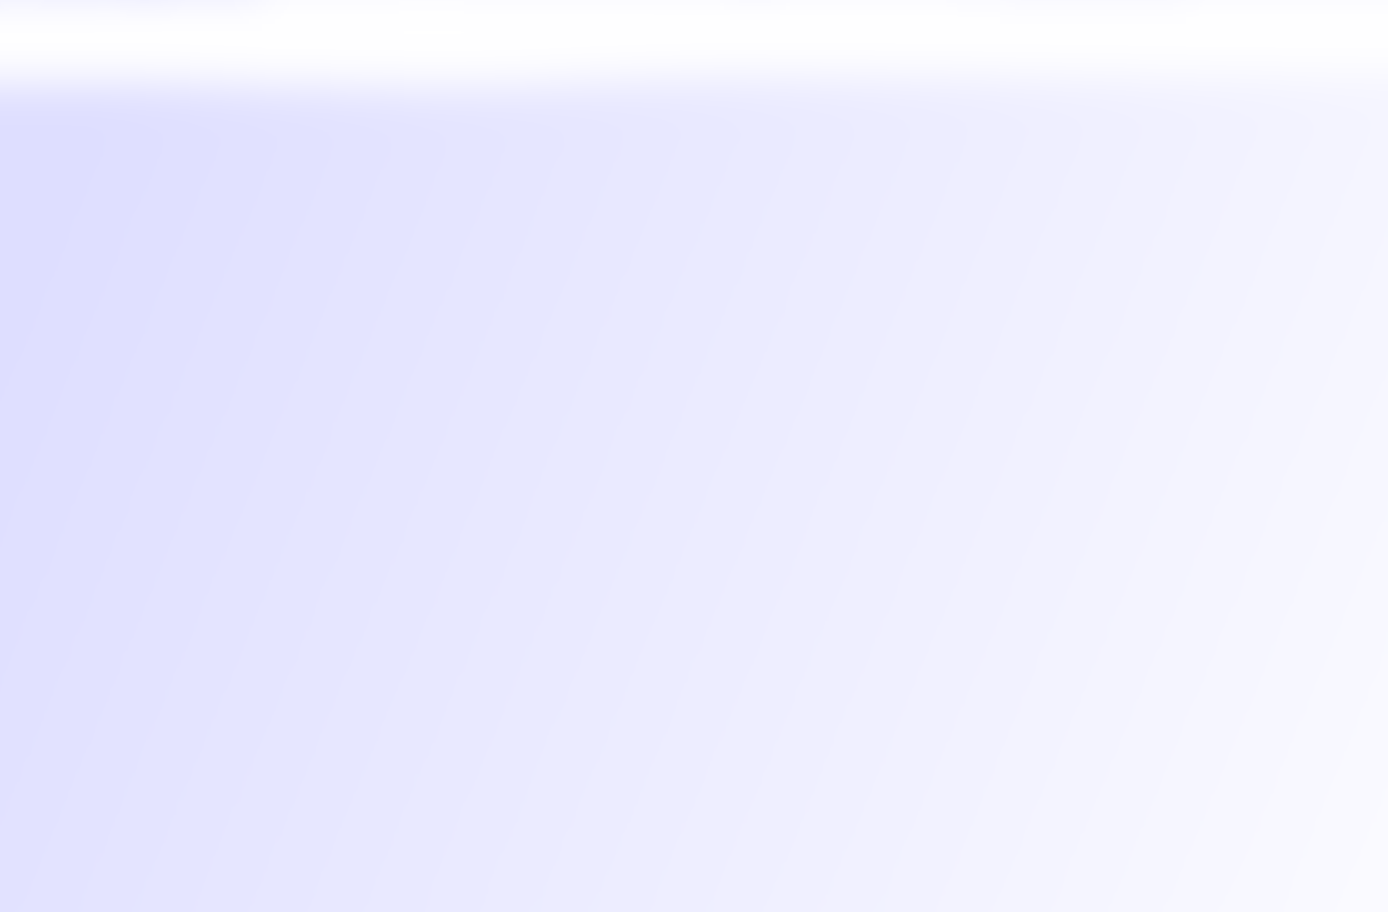
\includegraphics[height=1.1\textheight]{silhouettes_background}};
  \end{tikzpicture}%
}

\newlength{\leftimgwidth}
\begin{poster}%
  {
  grid=false, % Show grid to help with alignment
  colspacing=1em, % Column spacing
  % columns=5,
  % Color style
  bgColorOne=white,
  bgColorTwo=lightestyellow,
  borderColor=APLighterGrey,
  headerColorOne=blueOSHWDem,
  headerColorTwo=APDarkRed,
  headerFontColor=black,
  boxColorOne=APVeryLighterGrey,
  boxColorTwo=lighteryellow,
  % Format of textbox
  textborder=roundedleft,
  % textborder=rectangle,
  % Format of text header
  eyecatcher=true,
  headerborder=open,
  headerheight=0.1\textheight,
  headershape=roundedright,
  headershade=plain,
  headerfont=\Large\textsf, %Sans Serif
  boxshade=plain,
  % background=shade-tb,
  background=plain,
  linewidth=2pt
  }
  % Eye Catcher
  {
  
\includegraphics[height=5em]{bricolabs_logo.png}
  } % No eye catcher for this poster. (eyecatcher=no above). If an eye catcher is present, the title is centered between eye-catcher and logo.
  % Title
  {\sf %Sans Serif
  %\bf% Serif
  REFERENCIA RÁPIDA ARDUINO}
  % Authors
  {\sf %Sans Serif
  % Serif
  \vspace{0.05em}
  \textsc{OSHWDem - 2014}


  }
  {
    
\includegraphics[height=5em]{OSHWI_color.png} % University logo
  }

  \tikzstyle{light shaded}=[top color=baposterBGtwo!30!white,bottom color=baposterBGone!30!white,shading=axis,shading angle=30]

  % Width of left inset image
     \setlength{\leftimgwidth}{0.78em+8.0em}

%%%%%%%%%%%%%%%%%%%%%%%%%%%%%%%%%%%%%%%%%%%%%%%%%%%%%%%%%%%%%%%%%%%%%%%%%%%%%%
%%% Now define the boxes that make up the poster
%%%---------------------------------------------------------------------------
%%% Each box has a name and can be placed absolutely or relatively.
%%% The only inconvenience is that you can only specify a relative position 
%%% towards an already declared box. So if you have a box attached to the 
%%% bottom, one to the top and a third one which should be in between, you 
%%% have to specify the top and bottom boxes before you specify the middle 
%%% box.
%%%%%%%%%%%%%%%%%%%%%%%%%%%%%%%%%%%%%%%%%%%%%%%%%%%%%%%%%%%%%%%%%%%%%%%%%%%%%%
    %
    % A coloured circle useful as a bullet with an adjustably strong filling
    \newcommand{\colouredcircle}[1]{%
      \tikz{\useasboundingbox (-0.2em,-0.32em) rectangle(0.2em,0.32em); \draw[draw=black,fill=baposterBGone!80!black!#1!white,line width=0.03em] (0,0) circle(0.18em);}}

%%%%%%%%%%%%%%%%%%%%%%%%%%%%%%%%%%%%%%%%%%%%%%%%%%%%%%%%%%%%%%%%%%%%%%%%%%%%%%
\headerbox{Estructura}{name=structure,column=0,row=0}{
%%%%%%%%%%%%%%%%%%%%%%%%%%%%%%%%%%%%%%%%%%%%%%%%%%%%%%%%%%%%%%%%%%%%%%%%%%%%%%
  \begin{tabular}{l}
    void \textbf{setup}()   \\
    void \textbf{loop}() \\
  \end{tabular}
}

%%%%%%%%%%%%%%%%%%%%%%%%%%%%%%%%%%%%%%%%%%%%%%%%%%%%%%%%%%%%%%%%%%%%%%%%%%%%%%
\headerbox{Control de flujo}{name=control_stuctures,column=0,below=structure}{
%%%%%%%%%%%%%%%%%%%%%%%%%%%%%%%%%%%%%%%%%%%%%%%%%%%%%%%%%%%%%%%%%%%%%%%%%%%%%%
  \begin{tabular}{l}
    \texttt{\textbf{if}(x<5)\{\}}  \\
    \texttt{\textbf{for}(int i = 0; i < 255 i++ )\{\}} \\
    \texttt{\textbf{while}((x < 6 )\{\}} \\
  \end{tabular}
}

%%%%%%%%%%%%%%%%%%%%%%%%%%%%%%%%%%%%%%%%%%%%%%%%%%%%%%%%%%%%%%%%%%%%%%%%%%%%%%
\headerbox{Sintaxis adicional}{name=further_syntax,column=0,below=control_stuctures}{
%%%%%%%%%%%%%%%%%%%%%%%%%%%%%%%%%%%%%%%%%%%%%%%%%%%%%%%%%%%%%%%%%%%%%%%%%%%%%%
  \begin{tabular}{l l}
    \textbf{$//$} &  comentario de linea \\
    \textbf{$/*..*/$} & comentario multilinea \\
  \end{tabular}
  \vspace{3pt}
  \begin{tabular}{l}
    \#define ANSWER 42  \\
    \#include <myLib.h> \\
  \end{tabular}
}

%%%%%%%%%%%%%%%%%%%%%%%%%%%%%%%%%%%%%%%%%%%%%%%%%%%%%%%%%%%%%%%%%%%%%%%%%%%%%%
\headerbox{Operadores}{name=general_operators,column=0,below=further_syntax}{
%%%%%%%%%%%%%%%%%%%%%%%%%%%%%%%%%%%%%%%%%%%%%%%%%%%%%%%%%%%%%%%%%%%%%%%%%%%%%%
  \begin{tabular}{l l}
    \textbf{$=$} &  asignación \\
    \textbf{$+,$ \hspace{2pt} $ - $} & suma, resta \\
    \textbf{$*,$ \hspace{2pt} $ /$} &  multiplicación, division \\
    \textbf{$\%$} & módulo \\
    \textbf{$==$} & igualdad \\
    \textbf{$!=$} & desigualdad \\
    \textbf{$<$} & menor que \\
    \textbf{$<=$} &  menor o igual que \\
    \textbf{$>$} & mayor que \\
    \textbf{$>=$} &  mayor o igual que \\
  \end{tabular}
}

%%%%%%%%%%%%%%%%%%%%%%%%%%%%%%%%%%%%%%%%%%%%%%%%%%%%%%%%%%%%%%%%%%%%%%%%%%%%%%
\headerbox{Operadores de bit}{name=bitwise,column=0,below=pointers}{
%%%%%%%%%%%%%%%%%%%%%%%%%%%%%%%%%%%%%%%%%%%%%%%%%%%%%%%%%%%%%%%%%%%%%%%%%%%%%%
  \begin{tabular}{l l}
    \textbf{$\&$} &  bitwise AND \\
    \textbf{$|$} & bitwise OR \\
    \textbf{$\wedge$} & bitwise XOR \\
    \textbf{$\sim$} & bitwise NOT\\
  \end{tabular}
}

%%%%%%%%%%%%%%%%%%%%%%%%%%%%%%%%%%%%%%%%%%%%%%%%%%%%%%%%%%%%%%%%%%%%%%%%%%%%%
\headerbox{Operadores compuestos}{name=compound,column=0,below=bitwise}{
%%%%%%%%%%%%%%%%%%%%%%%%%%%%%%%%%%%%%%%%%%%%%%%%%%%%%%%%%%%%%%%%%%%%%%%%%%%%%%
  \begin{tabular}{l l}
    \textbf{$++$} &  Increment\\
    \textbf{$--$} & Decrement \\
    suma, resta, multiplicacion, division, modulo \\
    y operadores de bit pueden ser compuestos \\
    \textbf{$+=$},\textbf{$-=$},\textbf{$*=$},\textbf{$/=$} \\
    \textbf{$\&=$},\textbf{$|=$},\textbf{$^=$},\textbf{$~=$} \\
    \textbf{$\%=$} \\
  \end{tabular}
  %% OTHER COLUMS FOLLOW THIS COLUMN (bottom alignment)!!
  \vspace{9pt}
}

%%%%%%%%%%%%%%%%%%%%%%%%%%%%%%%%%%%%%%%%%%%%%%%%%%%%%%%%%%%%%%%%%%%%%%%%%%%%%
%% COLUMN 2 STARTS HERE
%%%%%%%%%%%%%%%%%%%%%%%%%%%%%%%%%%%%%%%%%%%%%%%%%%%%%%%%%%%%%%%%%%%%%%%%%%%%%
\headerbox{Constantes}{name=constants,column=1}{
%%%%%%%%%%%%%%%%%%%%%%%%%%%%%%%%%%%%%%%%%%%%%%%%%%%%%%%%%%%%%%%%%%%%%%%%%%%%%
  \begin{tabular}{l}
    \texttt{HIGH, LOW} \\
    \texttt{INPUT, OUTPUT}  \\
    \texttt{true, false}  
    \vspace{3pt}\\
    53 : Decimal  \\
    B11010101 : Binary  \\
    0x5BA4 : Hexadecimal  \\
  \end{tabular}
}

%%%%%%%%%%%%%%%%%%%%%%%%%%%%%%%%%%%%%%%%%%%%%%%%%%%%%%%%%%%%%%%%%%%%%%%%%%%%%
\headerbox{Tipos de datos}{name=data_types,column=1,below=constants}{
%%%%%%%%%%%%%%%%%%%%%%%%%%%%%%%%%%%%%%%%%%%%%%%%%%%%%%%%%%%%%%%%%%%%%%%%%%%%%%
  \begin{tabular}{l l}
    \textbf{void} & \\
    \textbf{boolean} & 0, 1, false, true  \\
    \textbf{char} & e.g. 'a' -128 $\rightarrow$ 127  \\
    \textbf{unsigned char} & 0 $\rightarrow$ 255 \\
    \textbf{int} & -32.768 $\rightarrow$ 32.767  \\
    \textbf{unsigned int} & 0 $\rightarrow$ 65535  \\
    \textbf{long} & -2.147.483.648 $\rightarrow$ 2.147.483.647  \\
    \textbf{float} & -3,4028235E+38 $\rightarrow$ 3.402835E+38  \\
    \textbf{sizeof} (myint) & returns 2 bytes  \\
  \end{tabular}
}

%%%%%%%%%%%%%%%%%%%%%%%%%%%%%%%%%%%%%%%%%%%%%%%%%%%%%%%%%%%%%%%%%%%%%%%%%%%%%
\headerbox{Arrays}{name=arrays,column=1,below=data_types}{
%%%%%%%%%%%%%%%%%%%%%%%%%%%%%%%%%%%%%%%%%%%%%%%%%%%%%%%%%%%%%%%%%%%%%%%%%%%%%%
  \begin{tabular}{l}
    int myInts[6];  \\
    int myPins[]={2,4,8,5,6};  \\
    int myVals[6]={2,-4,9,3,5};  \\
  \end{tabular}
}

%%%%%%%%%%%%%%%%%%%%%%%%%%%%%%%%%%%%%%%%%%%%%%%%%%%%%%%%%%%%%%%%%%%%%%%%%%%%%
\headerbox{Strings}{name=strings,column=1,below=arrays}{
%%%%%%%%%%%%%%%%%%%%%%%%%%%%%%%%%%%%%%%%%%%%%%%%%%%%%%%%%%%%%%%%%%%%%%%%%%%%%%
  \begin{tabular}{l}
    char S1[15];  \\
    char S2[8]={'A','r','d','u','i','n','o'};  \\
    char S3[8]={'A','r','d','u','i','n','o','$\backslash$0'};  \\
    char S4[]=``Arduino'';  \\
    char S5[8] = ``Arduino'';  \\
    char S6[15] = ``Arduino'';  \\
  \end{tabular}
}

%%%%%%%%%%%%%%%%%%%%%%%%%%%%%%%%%%%%%%%%%%%%%%%%%%%%%%%%%%%%%%%%%%%%%%%%%%%%%
\headerbox{Conversión}{name=conversion,column=1,below=strings}{
%%%%%%%%%%%%%%%%%%%%%%%%%%%%%%%%%%%%%%%%%%%%%%%%%%%%%%%%%%%%%%%%%%%%%%%%%%%%%%
  \begin{tabular}{l l l}
    \textbf{char()} & \textbf{int()} &  \textbf{long()}\\
    \textbf{byte()} & \textbf{word()} &  \textbf{float()}\\
  \end{tabular}
}

%%%%%%%%%%%%%%%%%%%%%%%%%%%%%%%%%%%%%%%%%%%%%%%%%%%%%%%%%%%%%%%%%%%%%%%%%%%%%
\headerbox{Calificadores}{name=qualifiers,column=1,below=conversion,bottomaligned=compound}{
%%%%%%%%%%%%%%%%%%%%%%%%%%%%%%%%%%%%%%%%%%%%%%%%%%%%%%%%%%%%%%%%%%%%%%%%%%%%%%
  \begin{tabular}{l l}
    \textbf{static} &  Persist between calls\\
    \textbf{volatile} & Use RAM (nice for ISR) \\
    \textbf{const} & Mark read-only \\
    \textbf{PROGMEM} & Use flash memory\\
  \end{tabular}
}

%%%%%%%%%%%%%%%%%%%%%%%%%%%%%%%%%%%%%%%%%%%%%%%%%%%%%%%%%%%%%%%%%%%%%%%%%%%%%
%% COLUMN 2 STARTS HERE
%%%%%%%%%%%%%%%%%%%%%%%%%%%%%%%%%%%%%%%%%%%%%%%%%%%%%%%%%%%%%%%%%%%%%%%%%%%%%
\headerbox{Interrupciones}{name=interrupts,column=2}{
%%%%%%%%%%%%%%%%%%%%%%%%%%%%%%%%%%%%%%%%%%%%%%%%%%%%%%%%%%%%%%%%%%%%%%%%%%%%%%
  \begin{tabular}{l}
    \textbf{attachInterrupt}(interrupt, function, type)  \\
    \textbf{detachInterrupt}(interrupt)  \\
    \textbf{boolean}(interrupt)  \\
    \textbf{interrupts}()  \\
    \textbf{noInterrupts}()  \\
  \end{tabular}
}

%%%%%%%%%%%%%%%%%%%%%%%%%%%%%%%%%%%%%%%%%%%%%%%%%%%%%%%%%%%%%%%%%%%%%%%%%%%%%
\headerbox{E/S Avanzada}{name=advanced_io,column=2,below=interrupts}{
%%%%%%%%%%%%%%%%%%%%%%%%%%%%%%%%%%%%%%%%%%%%%%%%%%%%%%%%%%%%%%%%%%%%%%%%%%%%%%
  \begin{tabular}{l}
    \textbf{tone}(pin, freqhz)  \\
    \textbf{tone}(pin, freqhz, duration\_ms)  \\
    \textbf{noTone}(pin)  \\
    \textbf{shiftOut} (dataPin, clockPin, how, value)  \\
    unsigned long \textbf{pulseIn}(pin, [HIGH,LOW])  \\
  \end{tabular}
}

%%%%%%%%%%%%%%%%%%%%%%%%%%%%%%%%%%%%%%%%%%%%%%%%%%%%%%%%%%%%%%%%%%%%%%%%%%%%%
\headerbox{Tiempo}{name=time,column=2,below=advanced_io}{
%%%%%%%%%%%%%%%%%%%%%%%%%%%%%%%%%%%%%%%%%%%%%%%%%%%%%%%%%%%%%%%%%%%%%%%%%%%%%%
  \begin{tabular}{l l}
    unsigned long \textbf{millis()} &  50 days overflow\\
    unsigned long \textbf{micros()}  & 70 min overflow \\
    \textbf{delay}(ms) &  \\
    \textbf{delayMicroseconds}(us) & \\
  \end{tabular}
}

%%%%%%%%%%%%%%%%%%%%%%%%%%%%%%%%%%%%%%%%%%%%%%%%%%%%%%%%%%%%%%%%%%%%%%%%%%%%%
\headerbox{Matemáticas}{name=math,column=2,below=time}{
%%%%%%%%%%%%%%%%%%%%%%%%%%%%%%%%%%%%%%%%%%%%%%%%%%%%%%%%%%%%%%%%%%%%%%%%%%%%%%
  \begin{tabular}{l l l}
    \textbf{min}(x,y) & \textbf{max}(x,y) & \textbf{abs}(x) \\
    \textbf{sin}(rad) & \textbf{cos}(rad) & \textbf{tan}(rad) \\
  \end{tabular}

  \begin{tabular}{l}
    \textbf{pow}(base, exponent)  \\
    \textbf{map}(val, fromL, fromH, toL, toH) \\
    \textbf{constrain}(val, fromL, toH) \\
  \end{tabular}
}

%%%%%%%%%%%%%%%%%%%%%%%%%%%%%%%%%%%%%%%%%%%%%%%%%%%%%%%%%%%%%%%%%%%%%%%%%%%%%
\headerbox{Números Pseudo Aleatorios}{name=random,column=2,below=math}{
%%%%%%%%%%%%%%%%%%%%%%%%%%%%%%%%%%%%%%%%%%%%%%%%%%%%%%%%%%%%%%%%%%%%%%%%%%%%%%
  \begin{tabular}{l}
    \textbf{randomSeed}(seed)  \\
    long \textbf{random}(max)  \\
    long \textbf{random}(min, max)  \\
  \end{tabular}
}

%%%%%%%%%%%%%%%%%%%%%%%%%%%%%%%%%%%%%%%%%%%%%%%%%%%%%%%%%%%%%%%%%%%%%%%%%%%%%
\headerbox{Pines E/S}{name=pins,column=3}{
%%%%%%%%%%%%%%%%%%%%%%%%%%%%%%%%%%%%%%%%%%%%%%%%%%%%%%%%%%%%%%%%%%%%%%%%%%%%%
\begin{center}
  \begin{tabular}{l l l}
    & \textbf{Uno} &  \textbf{Mega}\\
    \# of IO & 14 + 6 &  54 + 11  \\
    Serial Pins 3 & 0 - RX,   1 -TX & RX1 $\rightarrow$ RX4 \\
    Interrupts & 2,3 & 2,3,18,19,20,21 \\
    PWM Pins & 5,6 - 9,10 - 3,11 & 0 $\rightarrow$ 13 \\
    SPI \tiny{(SS, MOSI, MISO, SCK)}& 10$\rightarrow$ 13 & 50$\rightarrow$ 53 \\
    I2C \tiny{(SDA, SCK)} & A4, A5 & 20,21 \\
  \end{tabular}
\end{center}
}


%%%%%%%%%%%%%%%%%%%%%%%%%%%%%%%%%%%%%%%%%%%%%%%%%%%%%%%%%%%%%%%%%%%%%%%%%%%%%
%% COLUMN 3 STARTS HERE
%%%%%%%%%%%%%%%%%%%%%%%%%%%%%%%%%%%%%%%%%%%%%%%%%%%%%%%%%%%%%%%%%%%%%%%%%%%%%


%%%%%%%%%%%%%%%%%%%%%%%%%%%%%%%%%%%%%%%%%%%%%%%%%%%%%%%%%%%%%%%%%%%%%%%%%%%%%%
\headerbox{E/S Analógica}{name=analog,column=3,below=pins}{
%%%%%%%%%%%%%%%%%%%%%%%%%%%%%%%%%%%%%%%%%%%%%%%%%%%%%%%%%%%%%%%%%%%%%%%%%%%%%%
  \begin{tabular}{l}
    \texttt{\textbf{analogReference}(\texttt{EXTERNAL, INTERNAL})}  \\
    \texttt{int \textbf{analogRead}(pin)}  \\
    \texttt{\textbf{analogWrite}(pin,valor)} & PWM \\
  \end{tabular}
}

%%%%%%%%%%%%%%%%%%%%%%%%%%%%%%%%%%%%%%%%%%%%%%%%%%%%%%%%%%%%%%%%%%%%%%%%%%%%%
\headerbox{E/S Digital}{name=digital,column=3,below=analog}{
%%%%%%%%%%%%%%%%%%%%%%%%%%%%%%%%%%%%%%%%%%%%%%%%%%%%%%%%%%%%%%%%%%%%%%%%%%%%%%
  \begin{tabular}{l}
    \texttt{\textbf{pinMode}(pin,[\texttt{INPUT,OUTPUT}])}  \\
    \texttt{\textbf{digitalWrite}(pin, value)}  \\
    \texttt{int \textbf{digitalRead}(pin)}  \\
  \end{tabular}
}

%%%%%%%%%%%%%%%%%%%%%%%%%%%%%%%%%%%%%%%%%%%%%%%%%%%%%%%%%%%%%%%%%%%%%%%%%%%%%
\headerbox{Comunicación Serie}{name=serial,column=3,below=digital}{
%%%%%%%%%%%%%%%%%%%%%%%%%%%%%%%%%%%%%%%%%%%%%%%%%%%%%%%%%%%%%%%%%%%%%%%%%%%%%%
  \begin{tabular}{l}
    \textbf{Serial.begin}(speed)  \\
    \textbf{Serial.print}(``Text'')  \\
    \textbf{Serial.println}(``Text'')  \\
  \end{tabular}
}

%%%%%%%%%%%%%%%%%%%%%%%%%%%%%%%%%%%%%%%%%%%%%%%%%%%%%%%%%%%%%%%%%%%%%%%%%%%%%
\headerbox{Web}{name=websites,column=3,below=serial}{
%%%%%%%%%%%%%%%%%%%%%%%%%%%%%%%%%%%%%%%%%%%%%%%%%%%%%%%%%%%%%%%%%%%%%%%%%%%%%%
  \begin{tabular}{l}
    \url{forum.arduino.cc}    \\
    \url{playground.arduino.cc} \\
    \url{arduino.cc/en/Reference}  \\
  \end{tabular}
}

%%%%%%%%%%%%%%%%%%%%%%%%%%%%%%%%%%%%%%%%%%%%%%%%%%%%%%%%%%%%%%%%%%%%%%%%%%%%%
\headerbox{Arduino Uno}{name=board,column=3,below=websites,bottomaligned=compound}{
%%%%%%%%%%%%%%%%%%%%%%%%%%%%%%%%%%%%%%%%%%%%%%%%%%%%%%%%%%%%%%%%%%%%%%%%%%%%%%
  \begin{center}
    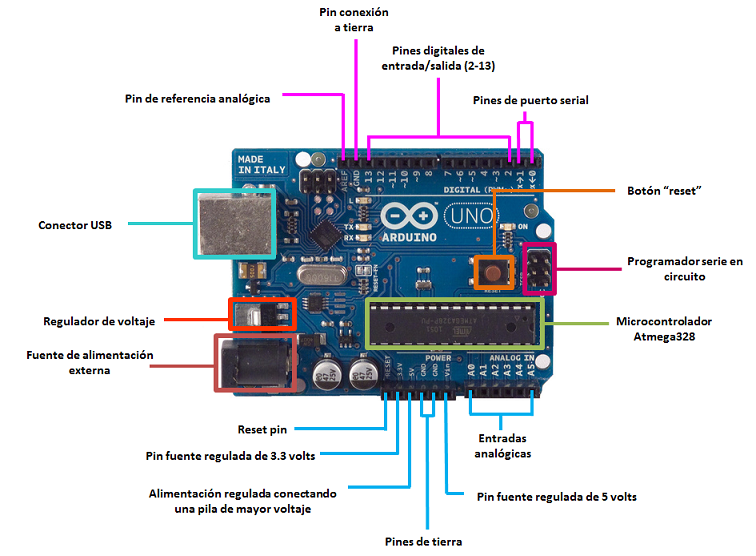
\includegraphics[width=0.95\textwidth]{./images/ARDUINO_UNO_PATAS.png}
  \end{center}
}



%%%%%%%%%%%%%%%%%%%%%%%%%%%%%%%%%%%%%%%%%%%%%%%%%%%%%%%%%%%%%%%%%%%%%%%%%%%%%%
\end{poster}
%%%%%%%%%%%%%%%%%%%%%%%%%%%%%%%%%%%%%%%%%%%%%%%%%%%%%%%%%%%%%%%%%%%%%%%%%%%%%%
\end{document}
%%%%%%%%%%%%%%%%%%%%%%%%%%%%%%%%%%%%%%%%%%%%%%%%%%%%%%%%%%%%%%%%%%%%%%%%%%%%%%
%%%%%%%%%%%%%%%%%%%%%%%%%%%%%%%%%%%%%%%%%%%%%%%%%%%%%%%%%%%%%%%%%%%%%%%%%%%%%%
